\documentclass[11pt]{article}
\usepackage[a4paper, total={6.8in, 9.25in}]{geometry}
\usepackage{graphicx}
\graphicspath{ {./assets/images/output/} }
\usepackage{caption}
\usepackage[english]{babel}
\usepackage{titling}
\usepackage{float}
\usepackage{amsmath}
\usepackage{minted}
\usepackage{multicol}
\usepackage{array}
\usepackage{setspace}
\usepackage{placeins}
\usepackage{tabularx}
\usepackage{booktabs}

% \usepackage{lipsum}

\title{Implementation of Static and RIP Routing in a Loop Configuration \& Simulations}
\author{}
\date{}

\pagenumbering{gobble}
\begin{document}
\input{cn_cover.tex}

\pagebreak

\tableofcontents

\pagebreak
\pagenumbering{arabic}
\maketitle

% --- Theory and Introduction ---
\section{Theory and Introduction}
Routing is the fundamental process of directing data packets across an interconnected network from a source node to a destination node through various intermediate devices. This experiment focuses on the Network Layer (Layer 3) of the Open Systems Interconnection (OSI) model \cite{tanenbaum2021}.

While linear or tree topologies are straightforward, they suffer from single points of failure. A loop topology introduces physical redundancy by providing multiple paths between any two nodes. In static routing, leveraging this redundancy requires the manual configuration of multiple pathways (e.g., equal-cost load balancing or floating static routes) so that if a primary link fails, an alternate path is predefined \cite{stallings2013}.

Dynamic routing addresses this automatically. The Routing Information Protocol (RIP) utilizes the Bellman-Ford algorithm to determine the best path based on hop count. In a loop configuration, if an active link fails, RIP dynamically recalculates the routing table and reroutes traffic through the surviving alternate paths without requiring manual administrative intervention, thereby providing superior fault tolerance \cite{tanenbaum2021}.

% --- Methodology ---
\section{Methodology}
The experiment was conducted using Cisco Packet Tracer (Version 9.0) \cite{packettracer2026}. A redundant loop topology was designed and tested in both static and dynamic environments through the following steps:

\begin{itemize}
    \item \textbf{Topology Construction:} A loop network was constructed utilizing three routers (Router0, Router1, Router2) interconnected via serial links (40.0.0.0, 50.0.0.0, and 70.0.0.0 networks). Three Local Area Networks (10.0.0.0, 20.0.0.0, and 30.0.0.0) were connected to the respective routers.
    \item \textbf{Phase 1 - Static Routing:} Static routes were manually configured. To utilize the loop's redundancy, multiple "Next Hop" routes were assigned for the same destination to facilitate alternative pathing.
    \item \textbf{Phase 2 - RIP Integration:} The static routes were removed, and the dynamic RIP routing process (\texttt{version 2}) was activated on all routers using the \texttt{network} command to advertise directly connected subnets.
    \item \textbf{Phase 3 - Fault Simulation:} A physical link failure was simulated by bringing down the connection between Router0 and Router1 in the RIP environment.
    \item \textbf{Verification:} End-to-end connectivity was evaluated using the \textit{Ping} utility in the static state, the optimal RIP state, and the faulty RIP state to verify network convergence and resilience.
\end{itemize}

% --- Results ---
\section{Results}
The comprehensive addressing scheme for the loop network is summarized in Table 1.

\begin{table}[h!]
    \centering
    \caption{Loop Network Addressing Table}
    \begin{tabular}{@{}lllll@{}}
        \toprule
        \textbf{Device} & \textbf{Interface} & \textbf{IPv4 Address} & \textbf{Subnet Mask} & \textbf{Default Gateway} \\ \midrule
        Router 0        & Fa0/0              & 10.10.10.0            & 255.0.0.0            & N/A                      \\
        Router 0        & Se2/0              & 40.40.40.1            & 255.0.0.0            & N/A                      \\
        Router 0        & Se3/0              & 70.70.70.1            & 255.0.0.0            & N/A                      \\
        Router 1        & Fa0/0              & 20.20.20.0            & 255.0.0.0            & N/A                      \\
        Router 1        & Se2/0              & 40.40.40.2            & 255.0.0.0            & N/A                      \\
        Router 1        & Se3/0              & 50.50.50.1            & 255.0.0.0            & N/A                      \\
        Router 2        & Fa0/0              & 30.30.30.0            & 255.0.0.0            & N/A                      \\
        Router 2        & Se2/0              & 50.50.50.2            & 255.0.0.0            & N/A                      \\
        Router 2        & Se3/0              & 70.70.70.2            & 255.0.0.0            & N/A                      \\
        PC 11           & NIC                & 10.10.10.1            & 255.0.0.0            & 10.10.10.0               \\
        Laptop 12       & NIC                & 10.10.10.2            & 255.0.0.0            & 10.10.10.0               \\
        PC 13           & NIC                & 10.10.10.3            & 255.0.0.0            & 10.10.10.0               \\
        PC 21           & NIC                & 20.20.20.1            & 255.0.0.0            & 20.20.20.0               \\
        Laptop 22       & NIC                & 20.20.20.2            & 255.0.0.0            & 20.20.20.0               \\
        PC 23           & NIC                & 20.20.20.3            & 255.0.0.0            & 20.20.20.0               \\
        PC 31           & NIC                & 30.30.30.1            & 255.0.0.0            & 30.30.30.0               \\
        PC 32           & NIC                & 30.30.30.2            & 255.0.0.0            & 30.30.30.0               \\
        PC 33           & NIC                & 30.30.30.3            & 255.0.0.0            & 30.30.30.0               \\ \bottomrule
    \end{tabular}
\end{table}

\begin{figure}[H]
    \centering
    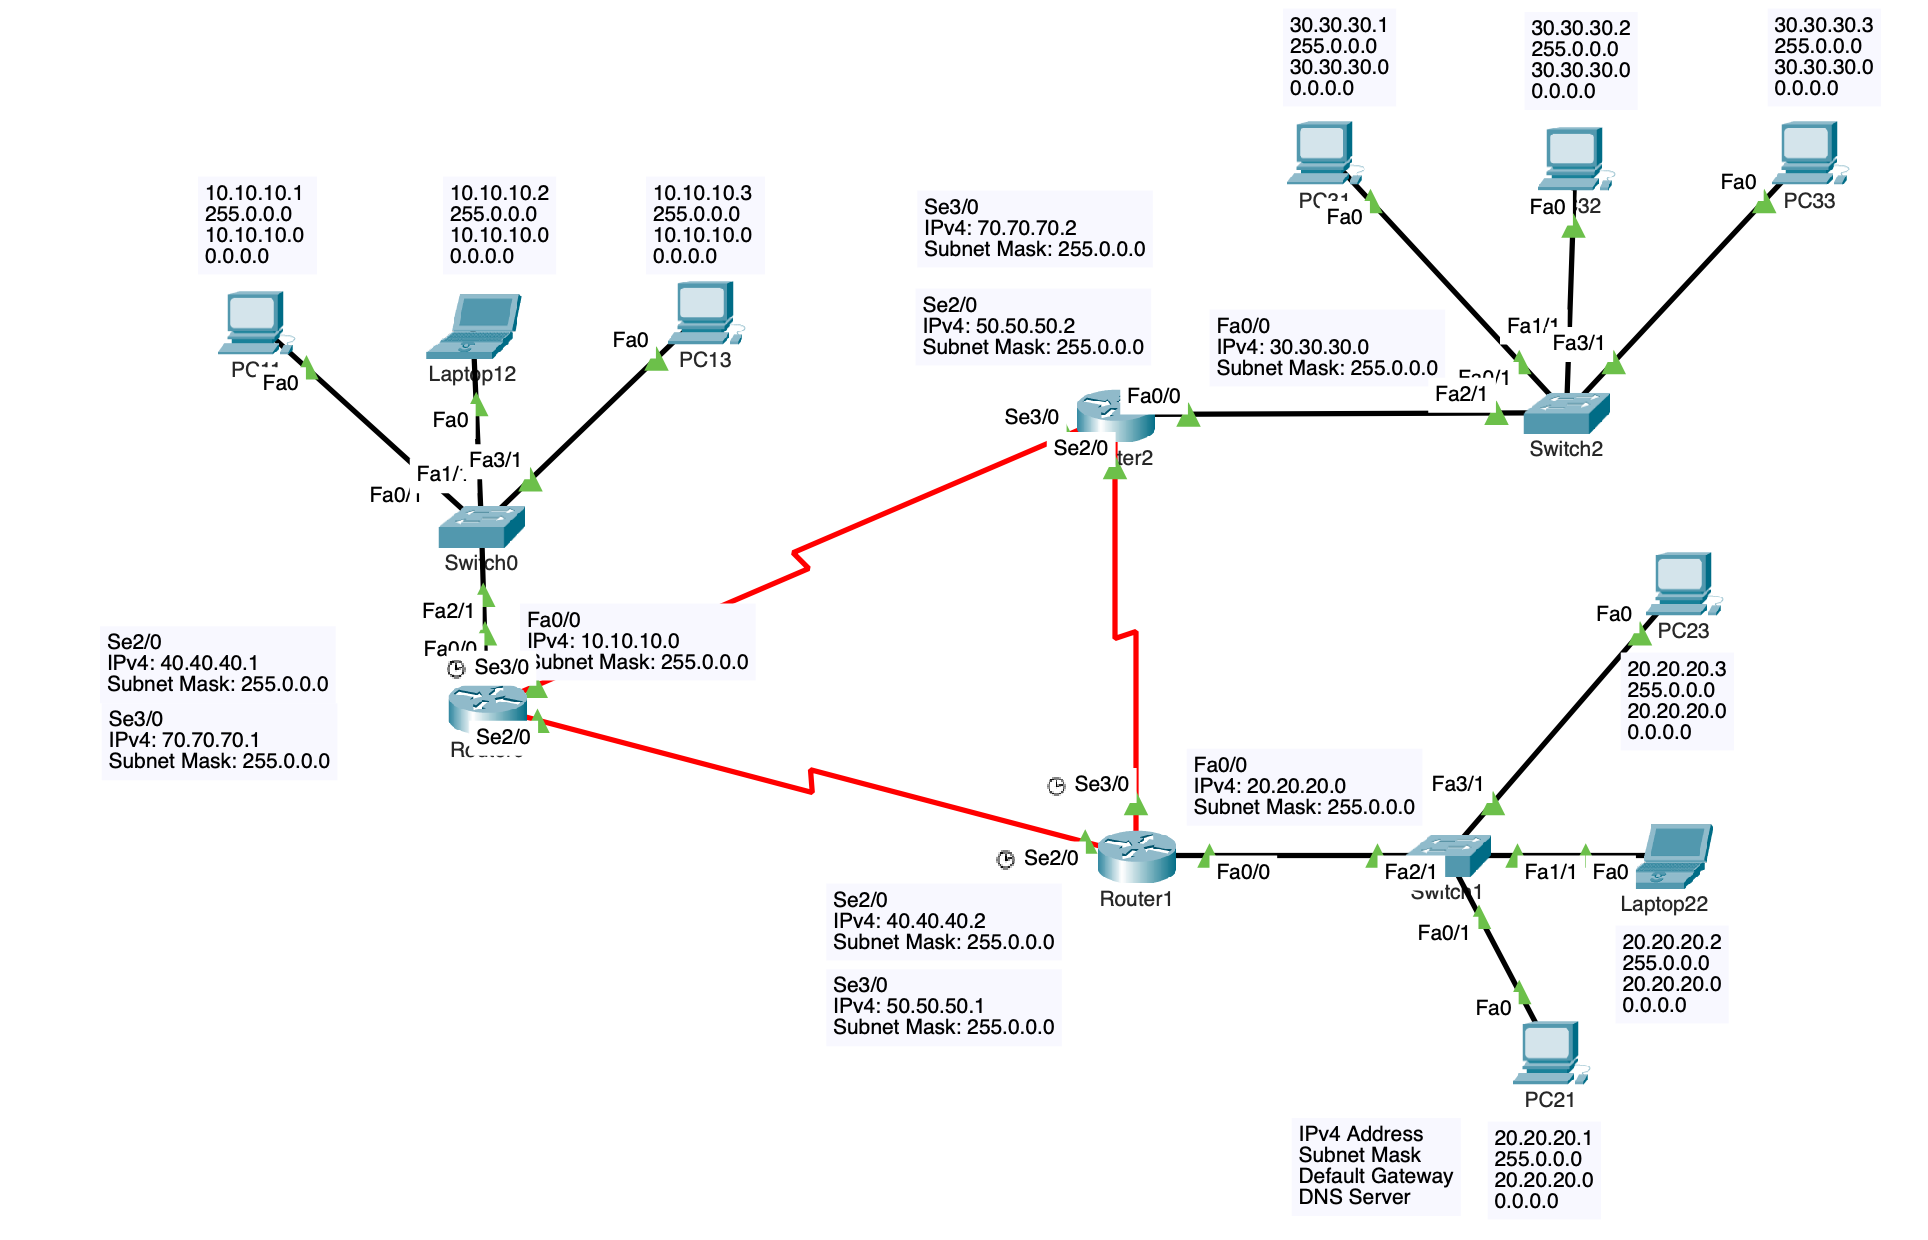
\includegraphics[width=0.85\textwidth]{static_network.png}
    \caption{Static Routing Loop Topology}
\end{figure}

\begin{figure}[H]
    \centering
    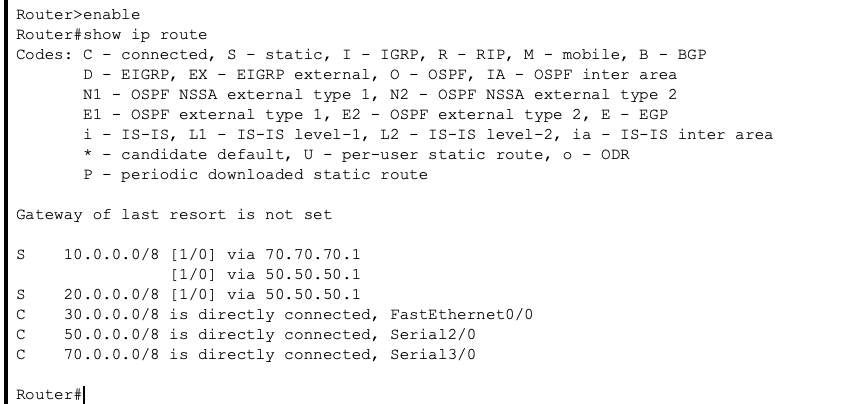
\includegraphics[width=0.85\textwidth]{static_route.png}
    \caption{Router 2 CLI: Static Routing Table displaying Redundant Paths}
\end{figure}

\begin{figure}[H]
    \centering
    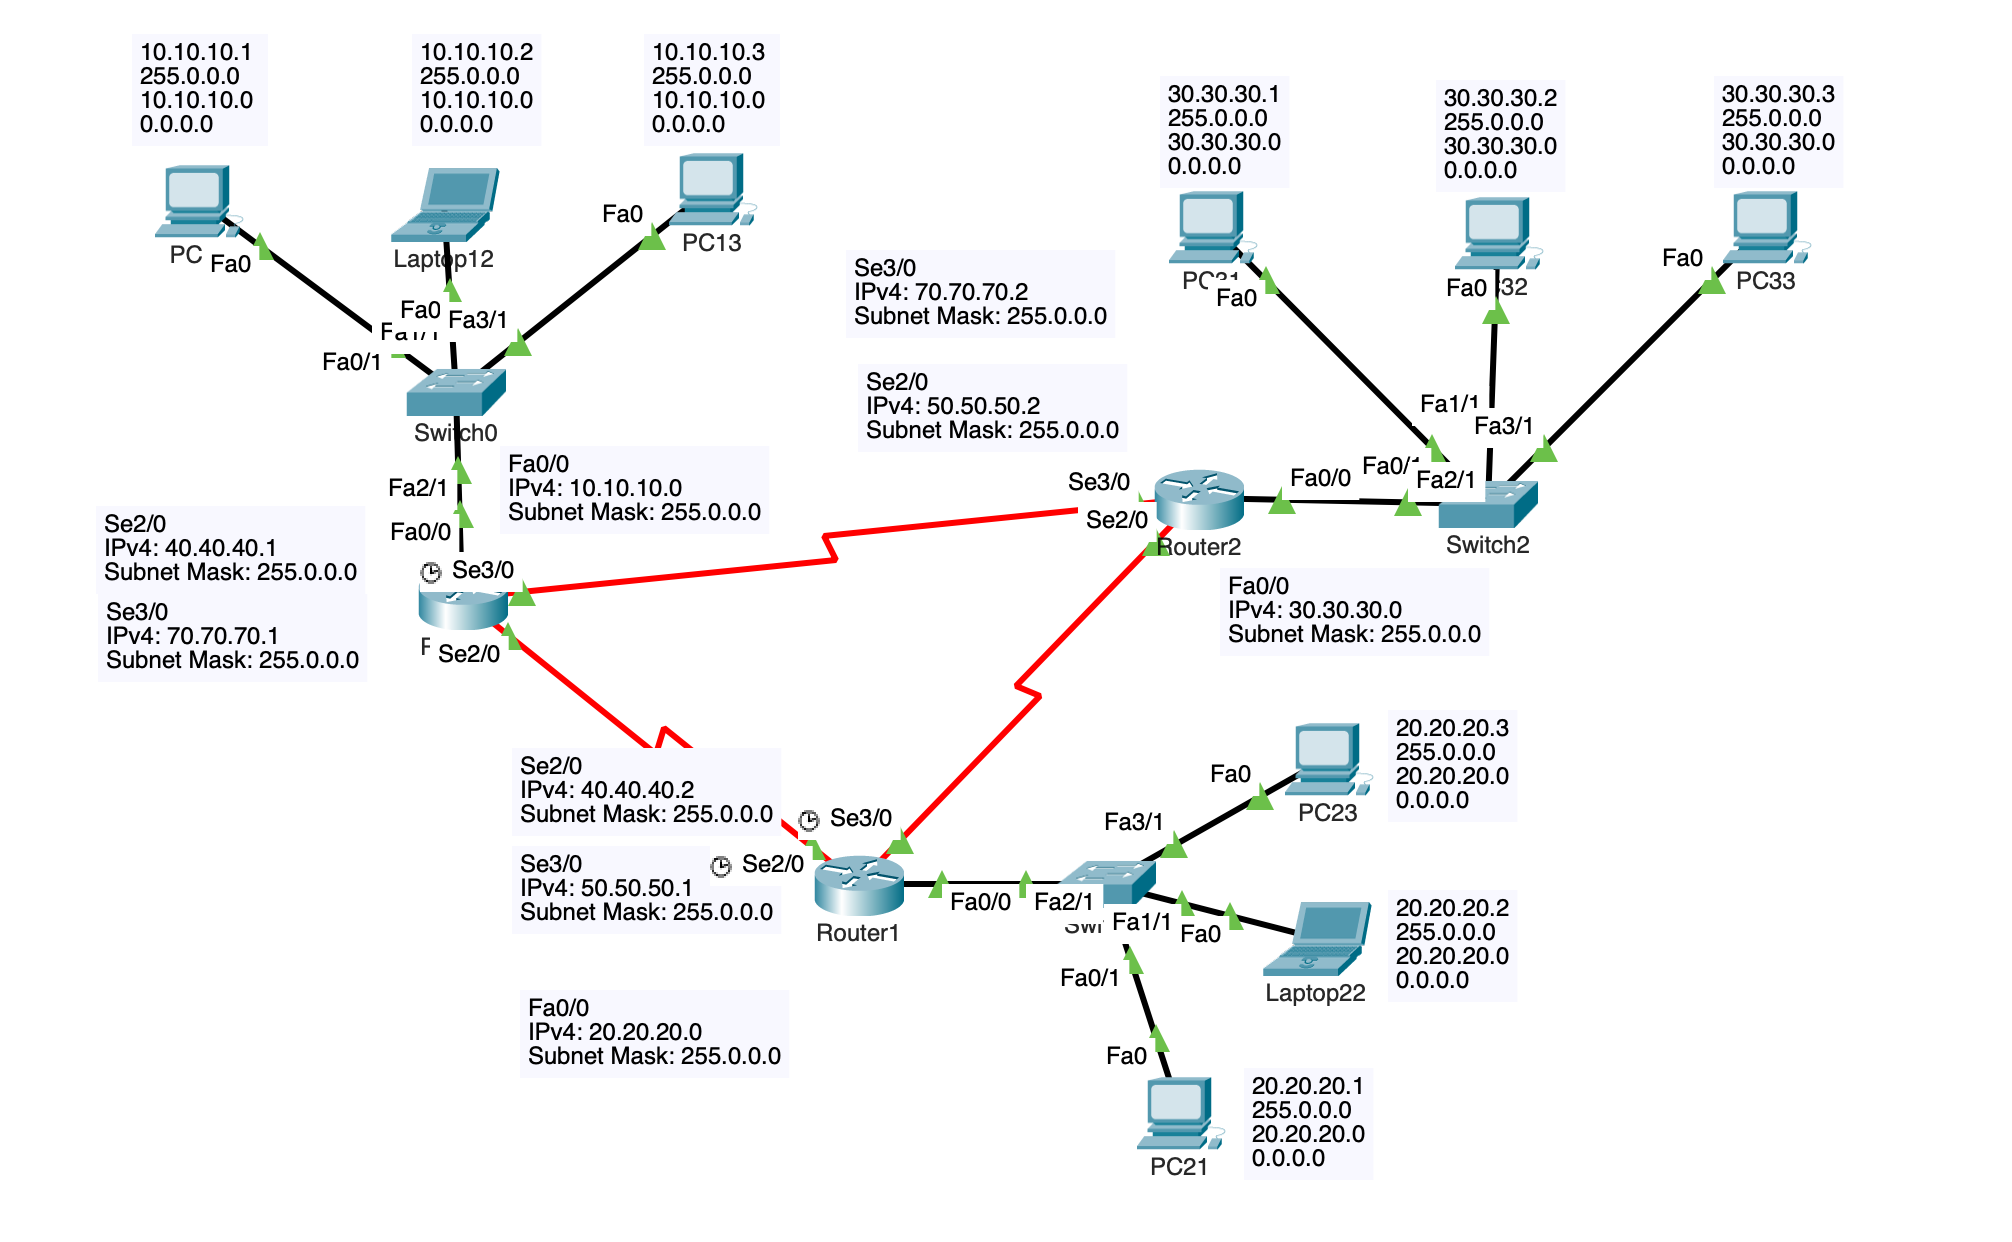
\includegraphics[width=0.85\textwidth]{rip_loop_network.png}
    \caption{Dynamic RIP Loop Topology (Optimal State)}
\end{figure}

\begin{figure}[H]
    \centering
    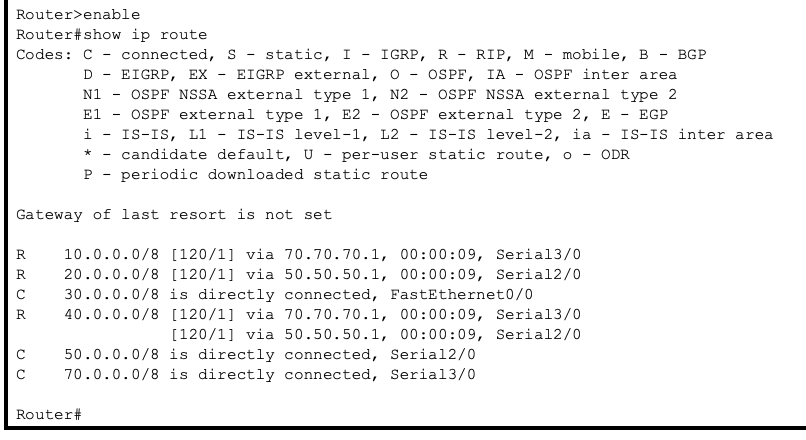
\includegraphics[width=0.85\textwidth]{rip_loop_route.png}
    \caption{RIP Routing Table (Optimal): Demonstrating Equal-Cost Load Balancing to 40.0.0.0/8}
\end{figure}

\begin{figure}[H]
    \centering
    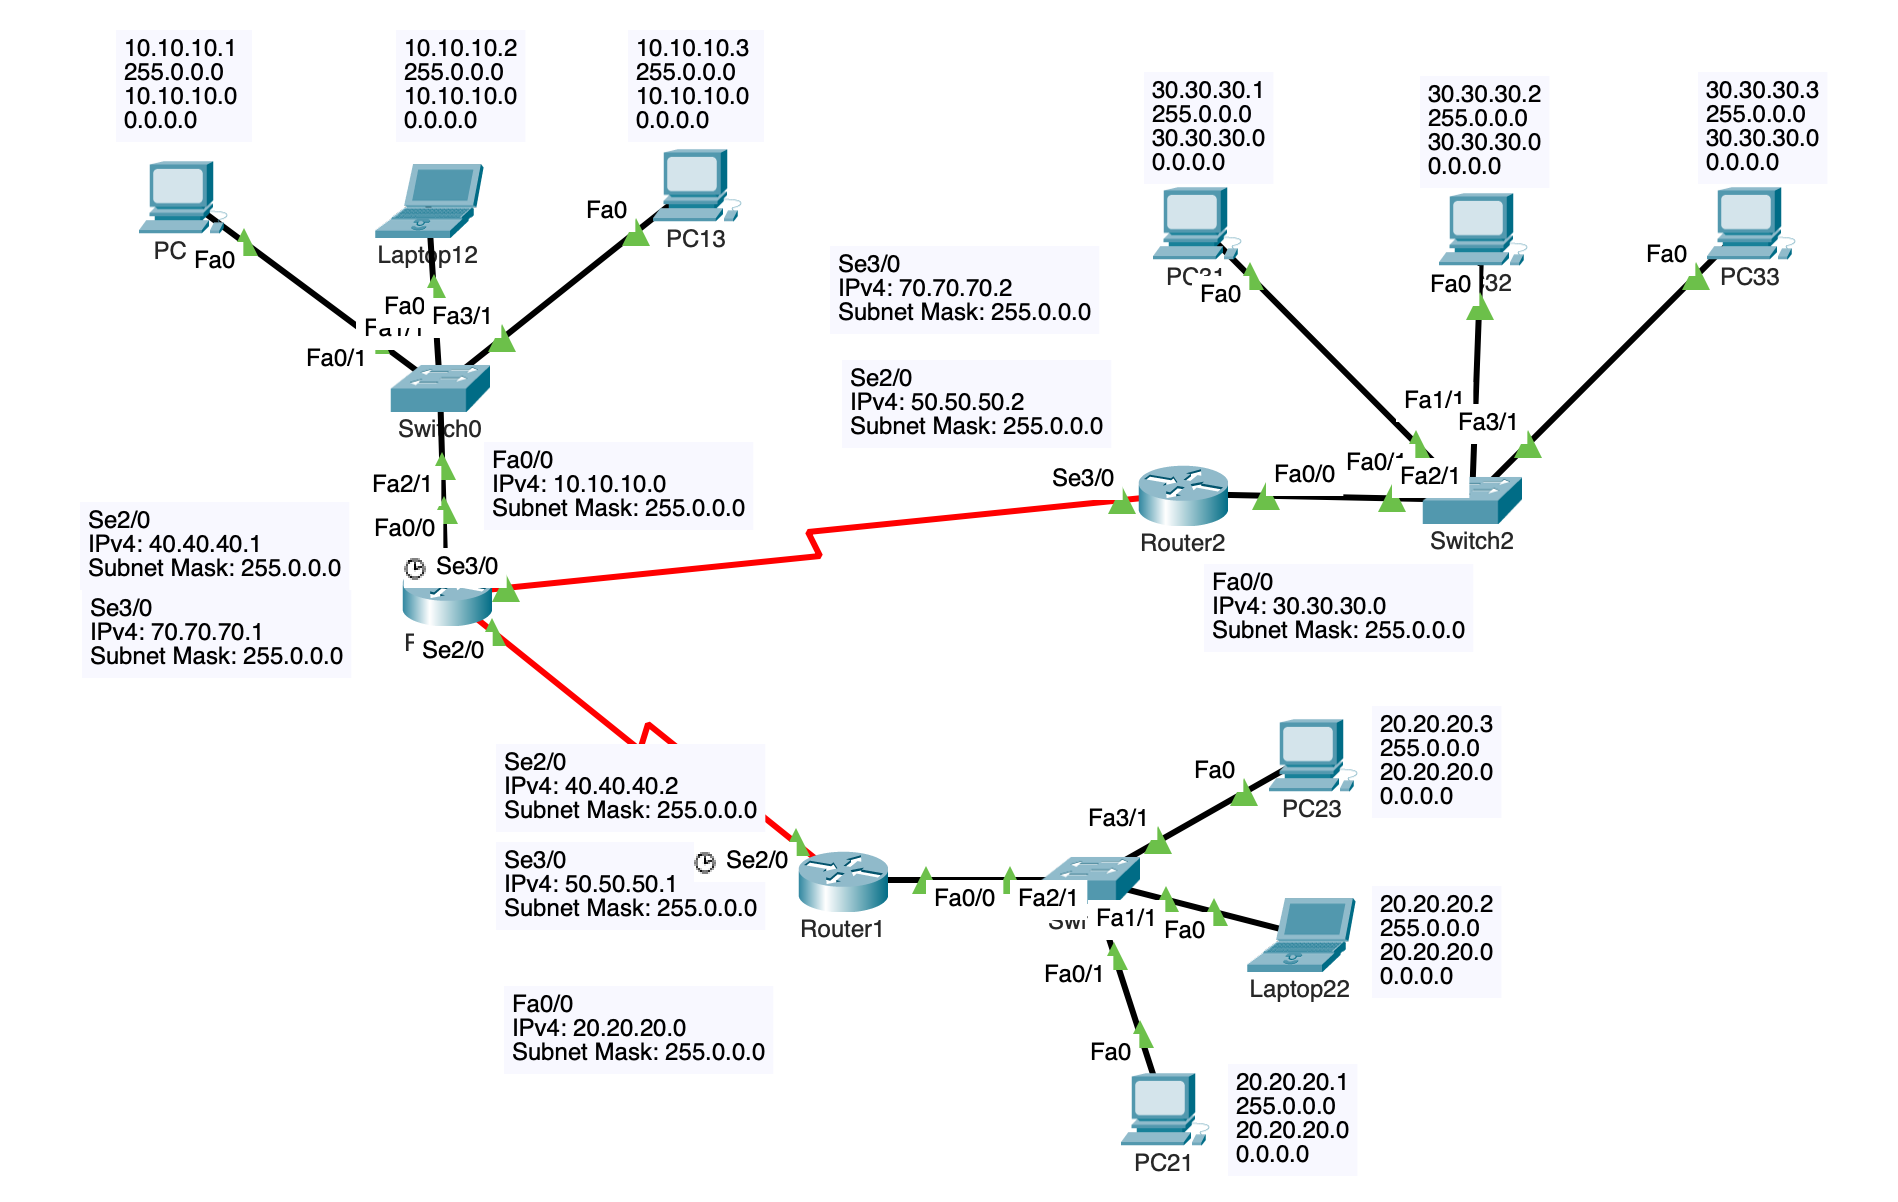
\includegraphics[width=0.85\textwidth]{rip_faulty_network.png}
    \caption{Dynamic RIP Loop Topology (Fault Simulated on Link 40.0.0.0)}
\end{figure}

\begin{figure}[H]
    \centering
    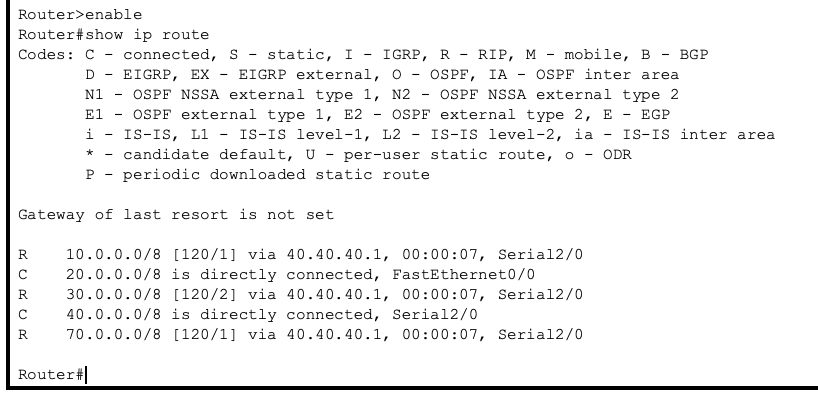
\includegraphics[width=0.85\textwidth]{rip_failty_route.png}
    \caption{RIP Routing Table (Fault State): Router 1 Dynamically Rerouting via Router 0}
\end{figure}

\begin{figure}[H]
    \centering
    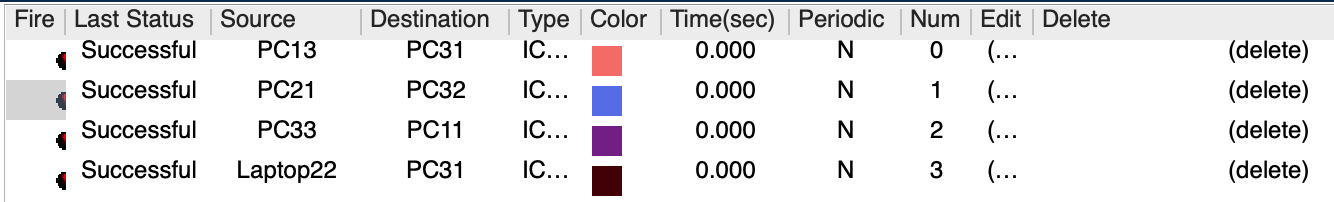
\includegraphics[width=0.85\textwidth]{rip_faulty_ping.png}
    \caption{Successful ICMP Verification during Link Failure}
\end{figure}

% --- Discussion ---
\section{Discussion}
The loop topology provided critical insights into network redundancy. During the static routing phase, the routing table for Router 2 (Figure 2) revealed that two explicit pathways were programmed to reach the 10.0.0.0 network: one directly via \texttt{70.70.70.1} and an alternate path via \texttt{50.50.50.1}. This demonstrated that fault tolerance in static environments requires rigorous, manual equal-cost configurations by the administrator.

Conversely, the implementation of the RIP protocol automated this redundancy. As observed in the optimal state (Figure 4), RIP not only found the shortest paths but also successfully performed load balancing. The routing table showed two active paths to the 40.0.0.0 network with an equal metric (hop count of 1), allowing the router to distribute traffic optimally.

The true resilience of the dynamic protocol was tested when the critical link (50.0.0.0 network) between Router 1 and Router 2 was intentionally severed (Figure 5). The protocol's self-healing capabilities were immediately evident in Router 1's updated routing table (Figure 6). Instead of dropping packets destined for the 30.0.0.0 network, RIP dynamically recalculated the path, routing the traffic through Router 0 (\texttt{via 40.40.40.1}) and reflecting an increased hop count of 2 (\texttt{[120/2]}). The subsequent simulation event list (Figure 7) confirmed successful message passing between nodes across the network, proving that RIP maintained seamless end-to-end connectivity during an unexpected physical link failure.

% --- Conclusion ---
\section{Conclusion}
The implementation of a loop topology was successfully achieved, demonstrating the importance of physical redundancy in network design. The simulations effectively contrasted static and dynamic routing approaches under failure conditions. While static routing can be forced into redundancy through manual equal-cost configurations, RIP proved highly superior in maintaining seamless end-to-end connectivity during unexpected link failures through automatic path recalculation.

\bibliographystyle{IEEEtran}
\renewcommand{\bibname}{References}
\addcontentsline{toc}{section}{References}
\bibliography{ref}

\end{document}
